\section{Methods}
\label{sec:method}

\subsection{From GNAN to weighted graphs}
In GNAN \citep{bechler2024gnan}, node features pass through learned shape functions and nodes
interact through a function of shortest-path distance. In a diagnostic on 20 evenly spaced
subjects from our cohort, median density was 0.498 and over 99.99\% of region pairs were one or two hops
apart. Hop distance therefore has little resolution here, while binarisation discards continuous
weights.

For transformed matrix $L$, let $s_i=\sum_jL_{ij}$, let $d_i$ be raw-support degree divided by
431, and let $w_{ij}=\mathrm{clip}(L_{ij}/q_{.99}^{\rm train},0,1)$. After train-fold
standardisation, W-GNAN (Figure~\ref{fig:method}) forms $u_i=f_i(s_i)+h(d_i)$, with region-specific $f_i$ and shared $h$:
\begin{equation}
\begin{aligned}
\mathrm{neigh}_i&=n_i^{-1}\sum_jm_{ij}g(w_{ij})u_j,\\
n_i&=\max(1,\sum_jm_{ij}).
\end{aligned}
\end{equation}
where the implemented interaction mask is $m_{ij}=\mathbf1[L_{ij}>0]$. The monotone piecewise-linear
$g$ has nine knots; positive softplus increments are cumulatively summed and normalized, enforcing
$g(0)=0,g(1)=1$. It starts at the identity, while $\lambda=\mathrm{softplus}(a)\geq0$ starts at 1.
Then $t_i=u_i+\lambda\mathrm{neigh}_i$ and $\ell=b+\sum_it_i$. Each $f_i$ has seven knots on
$[-3,3]$, $h$ has nine, and their knot values and the bias start at zero; all node shapes are anchored
at zero input. No self-loops are supplied; an isolate has zero neighbour term. The binary-topology
and fixed-linear ablations replace $g$ by
$\mathbf1[w>0]$ and $w$, respectively.

\begin{figure}[t]
\centering
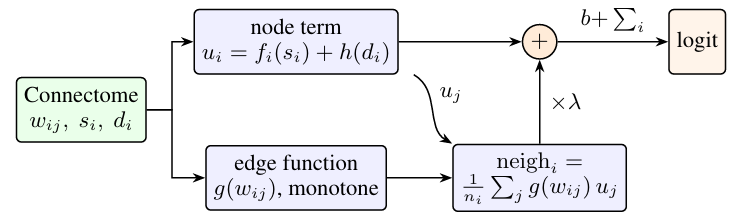
\includegraphics[width=\columnwidth]{figures/fig1_method.png}
\caption{W-GNAN. Strength and degree are graph-derived. The pairwise quantity in
Eq.~\ref{eq:decomp} is an interaction contribution to the fixed-graph logit, not an edge-removal or
causal effect.}
\label{fig:method}
\end{figure}

\subsection{Exact fixed-graph decomposition}
For a symmetric graph without self-loops, regrouping the directed neighbour sums gives
\begin{equation}
\label{eq:decomp}
\begin{aligned}
\ell&=b+\sum_i u_i+\lambda\sum_{i<j}C_{ij},\\
C_{ij}&=m_{ij}g(w_{ij})\left(u_j/n_i+u_i/n_j\right).
\end{aligned}
\end{equation}
This identity explains the model's \emph{logit for the observed fixed graph}. It is not a probability
decomposition, intervention, or causal claim. Moreover, changing/removing an edge can change $s_i$
and $d_i$, hence $u_i$; $C_{ij}$ is therefore the explicit interaction term, not the entire
perturbation effect of tract $(i,j)$. The region allocation $t_i$ and pairwise $C_{ij}$ are distinct
explanatory objects.

\paragraph{Property 1 (specified binary reference).} If the supplied weights and mask agree and
$w_{ij}\in\{0,1\}$, the endpoint constraints make $\mathrm{neigh}_i$ the mean of $u_j$ over
one-hop neighbours. W-GNAN then equals the mean-aggregating, one-hop GNAN variant used here; this is
not an equivalence claim for every GNAN configuration.

